%#MAKEINDEX makeindex interim01
\documentclass[10pt,a4j]{jarticle}

\newcommand{\setcounters}[1] {
  \setcounter{equation}{#1}
  \setcounter{figure}{#1}
  \setcounter{table}{#1}
}

\newcommand{\unit}[1] {
  \hspace{1mm}\mathrm{[#1]}
}

\newcommand{\degc} {
  \hspace{1mm}\mathrm{[}{}^\circ\mathrm{C]}
}

\newcommand{\refig}[1]{図\ref{fig::#1}}
\newcommand{\refeq}[1]{式(\ref{eq::#1})}
\newcommand{\reftab}[1]{表\ref{tab::#1}}

\newcommand{\fig}[5] {
  \begin{figure}[#1]
    \begin{center}
      \includegraphics[width=#2\hsize]{#3}
    \end{center}
    \caption{#4}
    \label{fig::#5}
  \end{figure}
}

\makeatletter
\def\eq{\@ifstar\@eq\@@eq}
\def\@eq#1{\begin{equation*}#1\end{equation*}}
\def\@@eq#1#2{\begin{equation}#2\label{eq::#1}\end{equation}}
\makeatother

\newcommand{\diff}[2] {
  \frac{\mathrm{d}#1}{\mathrm{d}#2}
}

\newcommand{\pdiff}[2] {
  \frac{\partial #1}{\partial #2}
}


\newcommand{\ddt}[2][1] {
  \ifnum #1 < 2
    \frac{\mathrm{d}#2}{\mathrm{d}t}
  \else
    \frac{\mathrm{d}^#1#2}{\mathrm{d}t^#1}
  \fi
}

\newcommand{\e}[1] {
  \mathrm{e}^{#1}
}

\newcommand{\lparen}{(}
\catcode `( = \active
\newcommand{(}{\ifmmode\left\lparen\else\lparen\fi}

\newcommand{\rparen}{)}
\catcode `) = \active
\newcommand{)}{\ifmmode\right\rparen\else\rparen\fi}

\newcommand{\bmat}[1] {
  \begin{bmatrix} #1 \end{bmatrix}
}

% -- Package ---------------------------------------------------
\usepackage[dvipdfmx]{graphicx}
\usepackage{amsmath, amssymb}
\usepackage{bm}
\usepackage{fancyhdr}
\usepackage{here}
\usepackage{listings}
\usepackage{multirow}


% -- Margin Config ---------------------------------------------
\setlength{\textheight}{\paperheight}
\setlength{\topmargin}{4.6truemm} % 30mm(=1.0in+4.6mm)
\addtolength{\topmargin}{-\headheight}
\addtolength{\topmargin}{-\headsep}
\addtolength{\textheight}{-60truemm}

\setlength{\textwidth}{\paperwidth}
\setlength{\oddsidemargin}{-0.4truemm} % 25mm(=1.0in-0.4mm)
\setlength{\evensidemargin}{-0.4truemm}
\addtolength{\textwidth}{-50truemm}


% -- Renewcommand ----------------------------------------------
\renewcommand{\theequation}{\arabic{section}.\arabic{equation}}
\renewcommand{\thefigure}{\thesection.\arabic{figure}}
\renewcommand{\thetable}{\thesection.\arabic{table}}
\renewcommand{\lstlistingname}{ソースコード}
\renewcommand{\headrulewidth}{0mm} % fancy
\renewcommand{\labelenumi}{(\arabic{enumi})}


% -- Config for fancy package ----------------------------------
\pagestyle{fancy}
\rhead{\thepage}
\lhead{}
\cfoot{}


% -- Config for package listings -------------------------------
\lstset{
  basicstyle={\ttfamily \small},
  breaklines=true,
  frame=trBL,
  numbers=left,
  numberstyle={\ttfamily \small},
}




\begin{document}

\def\maintitle{知能制御PBL\\}
\def\subtitle{最終報告書(個人レポート)\\}
\def\affiliation{九州工業大学 工学部 機械知能工学科\\知能制御工学コース 西田健研究室\\}

\def\dates{
  \hspace{0mm} 提出日:2017年08月08日 \\
}

\def\members{
      報告者:{\large 14104131} \hspace{1mm} 山崎 達也   \\
  共同実験者:{\large 13104042} \hspace{1mm} 烏谷 崇大   \\
              {\large 14104043} \hspace{1mm} 桑野 僚大   \\
              {\large 14104034} \hspace{1mm} 下松八重 宏太 \\
              {\large 14104090} \hspace{1mm} 中尾 真人   \\
              {\large 14104111} \hspace{1mm} 本田 空    \\
              {\large 16104313} \hspace{1mm} 山下 翔    \\
}

\begin{titlepage}
  \vspace*{25mm}
  \begin{center}
    {\huge \maintitle} \vspace{5mm}
    {\Huge \subtitle}  \vspace{20mm}
    {\Large \dates}
  \end{center}
  \vspace{25mm}
  \begin{flushright}
    {\LARGE \affiliation}
    \vspace{10mm}
    {\Large \members}
  \end{flushright}
\end{titlepage}




\newpage
\section{目的}
学部3年までに学習した制御理論や電気回路,
情報工学の知識を使って, 競技場内を自律的に走行するロボットカーの製作を行う.
各研究室でチーム一丸となってプロジェクトを進行し,
共同で課題を達成することの難しさや楽しさを学び,
情報工学の知識を使って, 競技場内を自律的に走行するロボットカーの製作を行う.
各研究室でチーム一丸となってプロジェクトを進行し,
共同で課題を達成することの難しさや楽しさを学び,
エンジニアとして仕事を進めるための素養を身に付ける.


\section{Robot Car Race(RCR)2017競技ルール}
\subsection{ルール概要}
競技場には黄色のポールや,火災に見立てた複数の赤色のポールが設置されている.
ポールに接触せず,できるだけ速やかに火災を鎮火させる
消防ロボットカー(ロボカー)を作成する.

\subsection{競技場詳細}
競技場の全体図を図\ref{course}に示し,以下に詳細を説明する.
\begin{enumerate}
  \item 競技場は板張りの床であり,縦・横ともに $5400\unit{mm}$である.

  \item 競技場には黄色の固定ポールと赤色の火災ポールが設置されており,
        スタートからゴールまで,固定ポールには接触,
        火災ポールには衝突することなく通過しなければならない.

  \item 火災ポールは青色の鎮火ポールに赤色の幕を被せたものであり,
        上部におもりなどを落としたり,幕を剥がしたりすることで,
        鎮火ポールに変化させる(このポールの製作も行うこと).

  \item スタート後は右手に固定ポールを見ながら直進し,
        消火活動開始区間まで移動しなければならない.消火活動開始区間に
        進入後は,右折し,火災ポールを発見し次第,消火にあたる.

  \item すべての火災ポールを消火して,鎮火ポールに変化させたのち,
        ゴール地点で停止する.

  \item 火災ポールの配置は競技ごとに異なる.
        また,鎮火ポールが存在することもある.

  \item ポールは直径 $80\unit{mm}$・高さ $120\unit{mm}$の中空パイプであり,
        黄・赤・青の色が付けられている.
\end{enumerate}

\begin{figure}[t]
  \begin{center}
    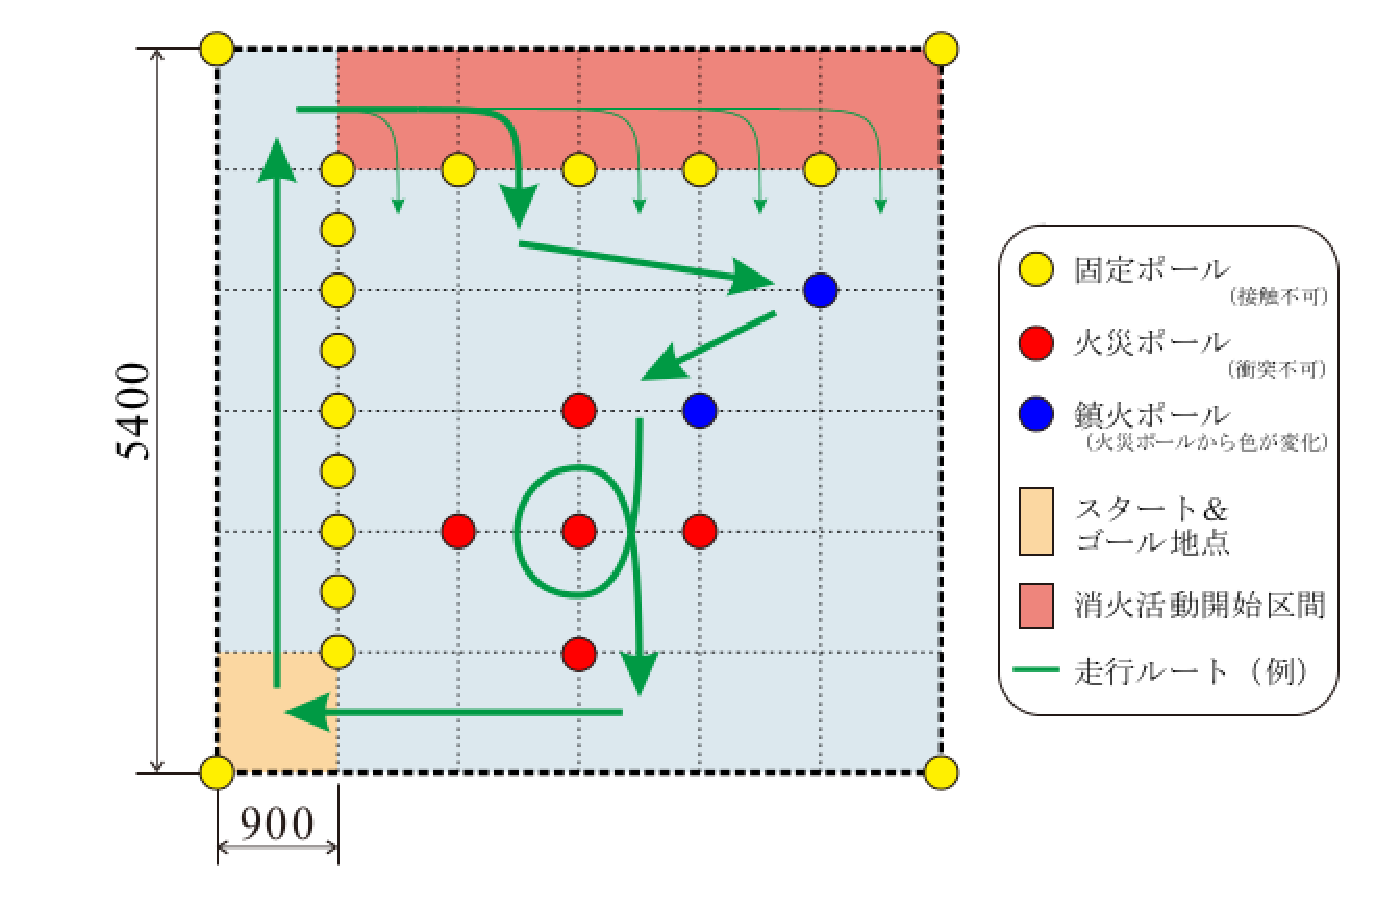
\includegraphics[width=1.0\hsize]{picture/course.eps}
    \caption{2017年度 RCR走行コース}
    \label{course}
  \end{center}
\end{figure}


\newpage
\section{ロボットカーの概要}
本年度のRCRでの我々の設計コンセプトは,
再現性の高い自律行動を可能にすることである,
そのために,ロボットカーには比較的構造が単純な独立二輪機構を採用する.
そして,赤・青・黄色ポールの色判別は,ロボット前方に取り付けた単眼カメラの映像を
画像処理することで行う,また,PSD(Position Sensitive Detector)センサと
赤外線近接センサを用いてポールとロボットの距離を測定することで,
適切な軌道の周回とポールの消火を目指す.
%ここに駆動輪の回転角度を検出するロータリエンコーダを用いた自己位置推定 
%(オドメトリ) と軌道追従制御を組み合わせた制御系を構成し,経路の完走を目指す.
製作にあたっては,研究室のメンバーをハードウェア,ソフトウェアの
担当に分けて進めることとする.


\section{消火について}
\subsection{消火ポール}
我々が用いる消火ポールは,以下のように製作する.\\
まず,塩化ビニル管に青い布を巻きつけて青いポールを作成する.
次に,青いポールの上から赤い布を覆うことで赤いポールとする.


\subsection{消火方法}
用いるポールの構造より,赤い布を青いポールから取り除くことで消火とする.
布を取り除く方法は,ロボットアームがポールの上から赤い布を
中に押し込んで,青いポールにするというものである.





\section{PSDセンサの同定実験}
\label{psdex}

前年度までに研究室で購入していた2種類のPSDセンサについて,
そのPSDセンサの精度を確かめるために同定実験を行った.

\subsection{センサの仕様}
前年度までに購入していた2種類のPSDセンサの仕様を以下に示す.
また,下記2つのセンサを便宜上,順に近距離センサ,長距離センサと
呼ぶこととする.\\

【シャープ測距モジュール GP2Y0A21YK】
  \begin{itemize}
   \item 測距範囲:$10〜80\unit{cm}$
   \item 出力:アナログ電圧出力
   \item 寸法:$29.5×13×13.5\unit{mm}$
   \item 電源:$4.5〜5.5\unit{V}$\\
  \end{itemize}

【シャープ測距モジュール GP2Y0A02YK】
  \begin{itemize}
   \item 測距範囲:$20〜150\unit{cm}$
   \item 出力:アナログ電圧出力
   \item 寸法:$29.5×13×21.6\unit{mm}$
   \item 電源:$4.5〜5.5\unit{V}$
  \end{itemize}

\subsection{実験装置}
PSDセンサの実験を行うため,図\ref{psded}のような実験装置を製作した.
PSDセンサは高さ$20\unit{mm}$の位置にセンサの発光部が左,
受光部が右になるように箱に水平に装着した.
PSDセンサを動作せるのにはArduino Unoを用い,
Arduino IDEのシリアルモニタを用いて出力電圧を測定した.
実験時のセンサとArduinoの配線を図\ref{psdwd}に,
Arduinoのプログラムを付録Aに示す.
配線にはブレッドボードを用いた.また,ポールの代わりに,
ポールと同じ形状のスプレー缶を用いた.

\begin{figure}[t]
  \begin{center}
   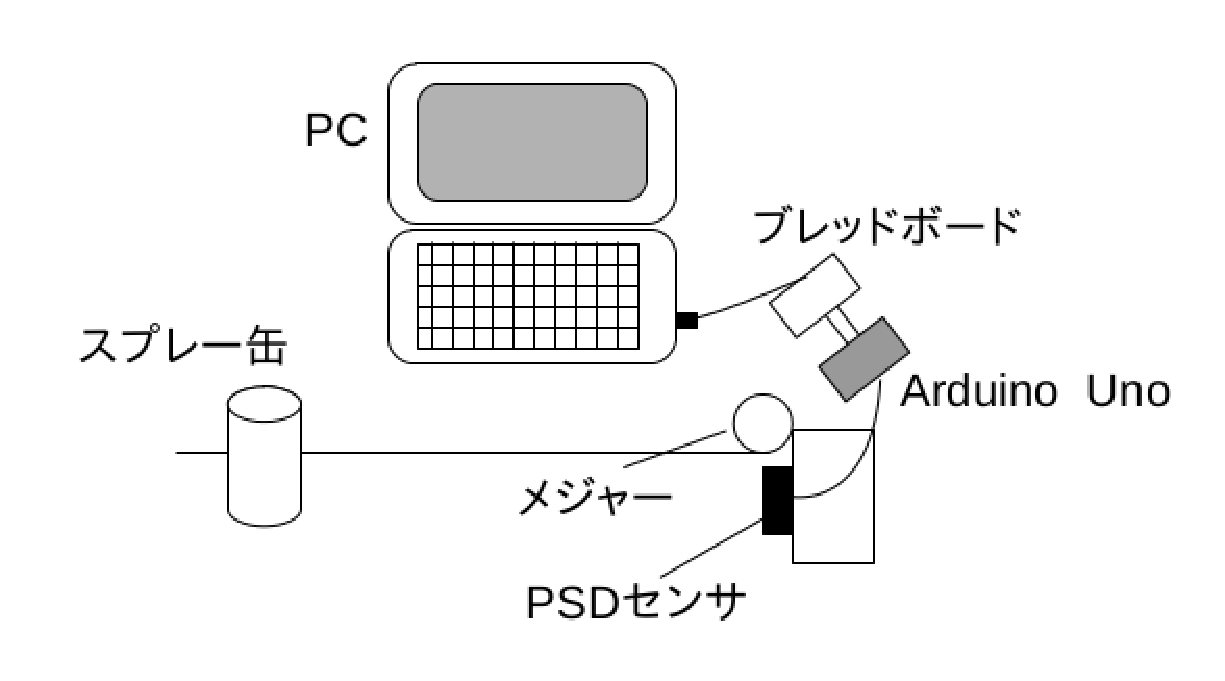
\includegraphics[scale = 0.8]{picture/psded.eps}
   \caption{PSD実験装置}
   \label{psded}
  \end{center}
\end{figure}

\begin{figure}
 \begin{center}   
  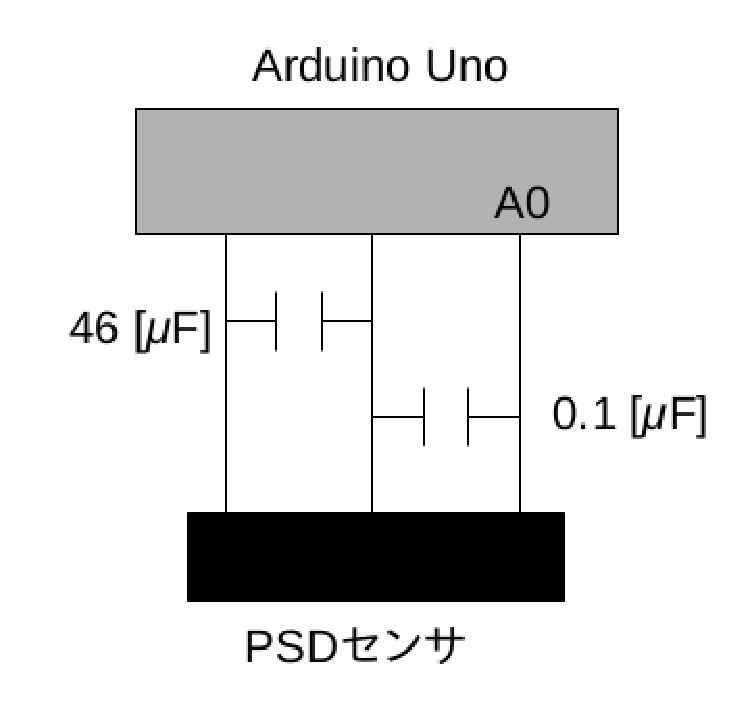
\includegraphics[scale = 0.8]{picture/psdwd.eps}
  \caption{PSDセンサの配線図}
  \label{psdwd}
 \end{center}
\end{figure}


\newpage
\subsection{実験方法}
PSDセンサの距離-出力電圧特性を測定するため以下の手順に従い実験を行った.
\begin{enumerate}
 \item PSDセンサの発光部・受光部の先端を距離$0\unit{cm}$とし,
       近距離センサは$5\unit{cm}$から$100\unit{cm}$まで,
       $5\unit{cm}$ずつスプレー缶を移動させ出力電圧を記録する.
       このとき,スプレー缶の中心はPSDセンサの中心の正面にくるように
       置き測定する.
 \item 先程と同様に,遠距離センサは$5\unit{cm}$から$170\unit{cm}$まで,
       $5\unit{cm}$ずつスプレー缶を移動させ出力電圧を記録する.
\end{enumerate} 

\subsection{実験結果}
縦軸を出力電圧,横軸をPSDセンサ-スプレー缶間の距離とし,
近距離センサの測定結果のグラフを図\ref{psdn}に,
長距離センサの測定結果のグラフを図\ref{psdf}に示す.
図\ref{psdn}より,近距離センサは出力電圧が$40\unit{cm}$までは
滑らかに減少しており,$40\unit{cm}$からは大きな変化は見られない.
それに対して図\ref{psdf}より,長距離センサは即距範囲内では
出力電圧が$80\unit{cm}$までは滑らかに減少しており,
$80\unit{cm}$からは値が上下しているが,大きな変化はないことがわかる.
大きな変化がない所は,どれくらい距離があるか区別できないため,
使用するべきではないと考えた.

よって,我々の考えるアルゴリズムに適当なセンサは,
$80\unit{cm}$まで距離の区別ができる長距離センサである.


\newpage
\begin{figure}[h]
  \begin{center}
    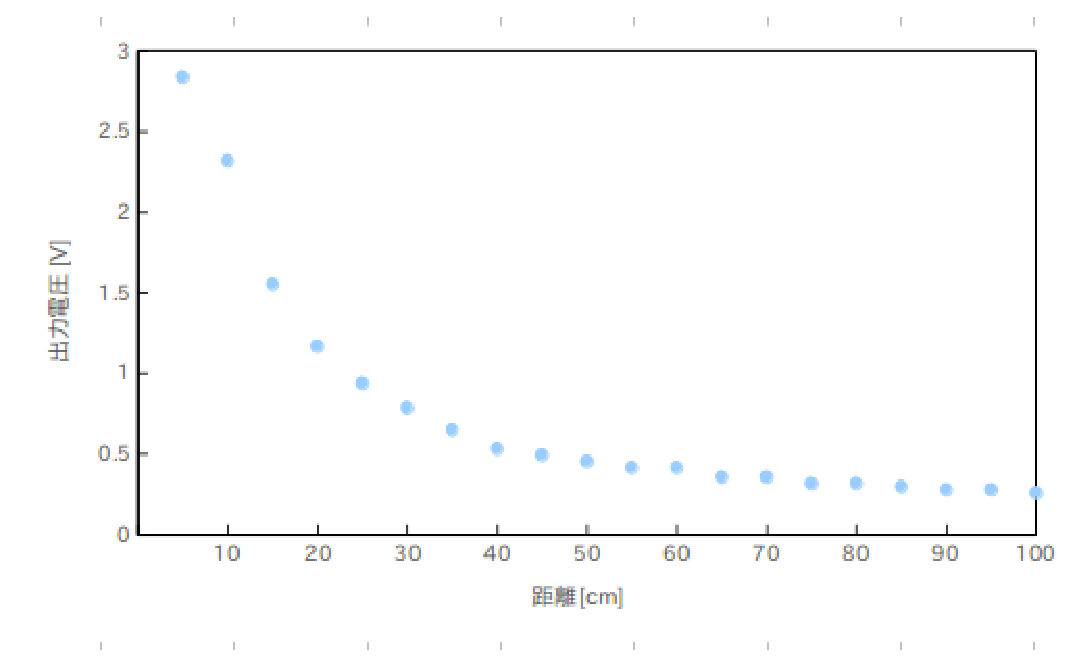
\includegraphics[width=1.0\hsize]{picture/psdn.eps}
    \caption{近距離センサ}
    \label{psdn}
  \end{center}
\end{figure}

\begin{figure}[h]
  \begin{center}
    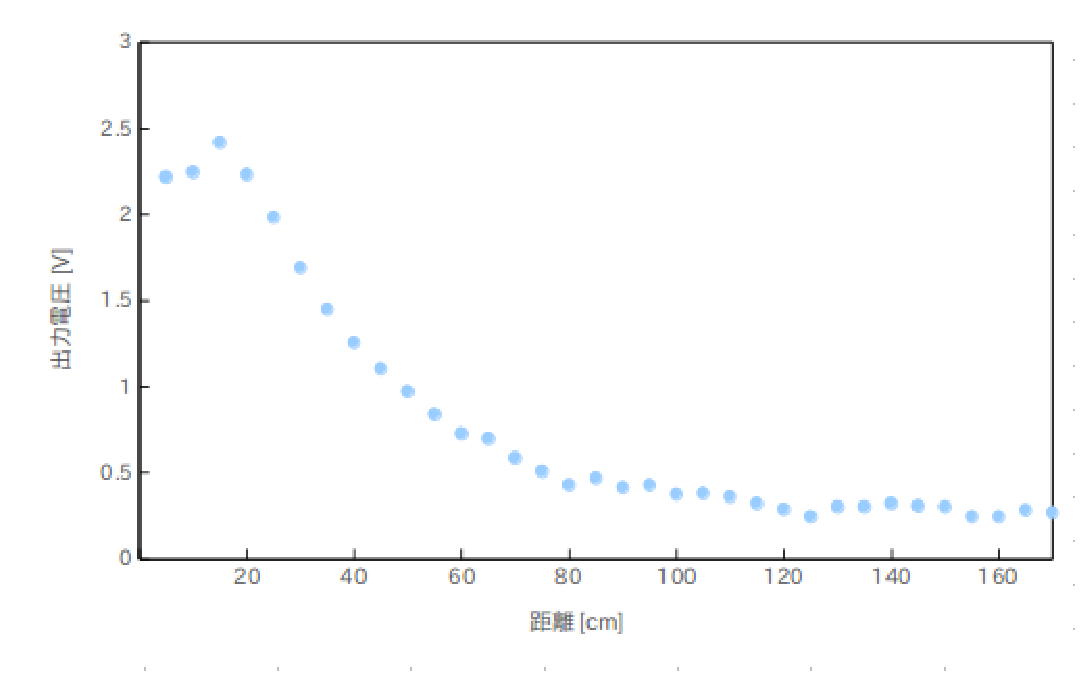
\includegraphics[width=1.0\hsize]{picture/psdf.eps}
    \caption{長距離センサ}
    \label{psdf}
  \end{center}
\end{figure}


\newpage
\subsection{PSDセンサの課題}
今回のRCRにおいて用いるPSDセンサの課題として,
実験により得られた測定値のデータにノイズが入ることが挙げられる.
これを改善するためにフィルタをかけてノイズを除去することを考える.
ここでは以下の2種類のフィルタについてその実用性を考察する.
ただし,それらの検証実験は今後行うものとする.

\subsubsection{平均値フィルタ}
実測値の中で範囲を決めて,その平均値をとるフィルタのことである.
ノイズの影響を小さくすることができるが,フィルタが長くなると応答性能が悪化する.

\subsubsection{メディアンフィルタ(中間値フィルタ)}
奇数個のデータの中間に位置する値をその位置のデータとして
採用するフィルタのことである.スパイクノイズを取り除くのに適しているため,
今回使用するPSDセンサにはこちらのフィルタを用いることが適切であると考えられる.


\end{document}
